\documentclass[english,a4paper,oneside]{article}%{scrartcl}

\usepackage[bookmarks=true,
citebordercolor={0 0.75 0},
filecolor=black,
linkbordercolor={1 1 1},
linkcolor={0 0 1},
pdfauthor={Jürgen Maier, Philipp Paulweber, Stefan Mödlhamer},
pdfmenubar=false,
urlbordercolor={1 1 1},
pdfborder={0 0 0},
pdftex]{hyperref}

\usepackage{url}
\usepackage[english]{babel}

\usepackage{ucs}
\usepackage[utf8x]{inputenc}


\usepackage{listings} 
\lstset{escapechar=?} 
\newcommand{\uc}[1]{ \scriptsize{\texttt{#1}} }

\usepackage{amsmath}
\usepackage{amsfonts}
\usepackage{amssymb}

\usepackage[pdftex]{graphicx}

\usepackage[nottoc,numbib]{tocbibind}
\usepackage{color}
\usepackage{soul}
\bibliographystyle{plain}

\title
{		
	\vspace{0mm}
	\begin{center}
		
\includegraphics[width=0.60\textwidth]{img/vtou.pdf}
	\end{center}
	\vspace{5mm}
	\Large{Computer Aided Verification}\\
	\large{181.144, UE, 2012S}\\	
	\vspace{10mm}
	%\Huge{\textbf{TinyC Interpreter}}\\
	\vspace{5mm}
	\begin{center}
		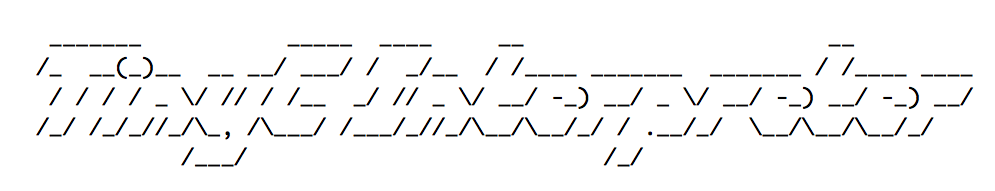
\includegraphics[width=1.0\textwidth]{img/logo.png}
	\end{center}	
	\huge{\textbf{User Manual}}\\
	\vspace{10mm}
}

\author
{ 
	\begin{tabular}{ll}
		Jürgen Maier        	&e0825749@student.tuwien.ac.at\\
		Philipp Paulweber		&e0727937@student.tuwien.ac.at\\
		Stefan Mödlhamer	&e0825895@student.tuwien.ac.at
	\end{tabular}
}

\date
{
	\vfill %\vspace{0mm}
	\today
	\vspace{10mm}
	\begin{tabular}{ll}
		Git Date:	& \texttt{2012-11-01 17:44:56}\\
		Git Tag:	& \texttt{Release, 1.0}\\
		Git Hash: 	&	\texttt{a31bf5aa4bc08cb865551c6c0d5d2eac4ef7329f}
	\end{tabular}
}

\begin{document}
\maketitle
\thispagestyle{empty}
\newpage
\tableofcontents

\newpage
%++++++++++++++++++++++++++++++++++++++++++++
\section{Overview}
This manual describes the behavior and the usage of the \emph{TinyC interpreter} which was developed during the exercise of the course ``Computer Aided Veri\- fication" \cite[p.~5]{cav}. The questions ``What is \emph{TinyC}?" and ``What is an \emph{interpreter}?" are answered at the beginning, followed by the description of the installation/compilation process. At the end the usage of the interpreter is described and outlined with some examples.

\subsection{TinyC}
TinyC is a small subset of the C programming language, defined at \cite[p.~4]{cav}. The correct version of the TinyC grammar in EBNF is in the appendix section at \ref{grammer}.\\

We used the term ``correct version" here because unfortunately the defined EBNF grammar contained an error and was corrected. However we found out later that even the corrected version is erroneous. The problem is an expression in the grammar which looked in the first version of the exercise sheet like this:

\begin{scriptsize}
\begin{lstlisting}
	<expr> ::= <test> | <id> "=" <expr> | "!" <expr>
\end{lstlisting}
\end{scriptsize}

The problem is that the parser structure of the interpreter can not clearly identify which lexical element should be used by the negation operator (\texttt{!}) -- \texttt{<test>} or an assignment (\texttt{<id> "=" <expr>}). Due to that problems the last transition was changed to:

\begin{scriptsize}
\begin{lstlisting}
	<expr> ::= <test> | <id> "=" <expr> | "!" <test>
\end{lstlisting}
\end{scriptsize}

However every expression in the C programming language can be negated, not only test elements, so we changed that into an expression surrounded by parentheses: 

\begin{scriptsize}
\begin{lstlisting}
	<expr> ::= <test> | <id> "=" <expr> | "!" <paren_expr>
  <paren_expr> ::= "(" <expr> ")"
\end{lstlisting}
\end{scriptsize}


\subsection{Interpreter}
An interpreter is a program that takes a source code file, in our case a TinyC source, and starts the analysis phase like a compiler. This phase consists of a lexer and a grammar parser, developed with the tools \texttt{flex}, \texttt{yacc} and \texttt{ox}.\\

After transforming the source code into an intermediate representation (IR), residing in the memory, \footnote{We used a classic abstract syntax tree (AST) transformation.} the interpreter converts the IR (AST) into a labeled transition system (LTS), which is afterwards used for calculations.

\subsubsection{Execution Modes}
There are two possible ways to interpret/calculate and execute a program:


\paragraph{Numeric Execution (default)}
is the default operation of the interpreter. For every defined input variable the interpreter requests an integer value from the user. If a variable is used in the source code and is not defined as input variable its starting value is defined as $0$.
%jürgen: i think that was what he meant, right?
%don't know what you mean by that
%\hl{If no input variable was defined in the source code, the default value is $0$.}
%
The calculations can either be performed in a \textit{free-run} or \textit{step-through} mode. In free-run the interpreter does the calculation in one step and outputs the value for each defined output variable. If no output variable was defined the message \textit{``no output variables declared"} will be printed instead. In the step-through mode only one transition on the LTS is done at once. That means that the program stops after each transition, printing the numeric values of the actual state and waiting for user actions. Available actions are to compute the next transition by pressing 'n' or abort the calculation with 'a'.


\paragraph{Symbolic Execution}
is an execution mode, where the user has to provide the interpreter an abstract trace (kripke structure) file\footnote{the format is defined in the appendix at \ref{tks} and based on the definition at \cite[p.~10]{cav}}, which is used to perform a symbolic evaluation on the LTS. Like in the previous described numeric execution mode the user is able to choose between a free-run or step-through calculation. The result of the calculation is either 'satisfiable', if the abstract trace is valid, or 'not satisfiable' if a non valid abstract trace was described. Furthermore the interpreter displays the counterexample symbolic formula if the trace was 'not satisfiable'.\\

All transition formulas and predicates of the abstract trace are checked with the SMT solver library ``MathSAT5" \cite{mathsat}.



%++++++++++++++++++++++++++++++++++++++++++++
\section{Compilation}
The installation process is quite simple: \texttt{make interpreter} compiles the interpreter right away and you are good to go. \\
Executing the Makefile with \texttt{make} (without options) shows the required dependencies needed to compile the project. Furthermore the README provides additional information.

\subsection{Build Dependencies}
In general it is possible to compile the project on every Unix/Linux system, however with the integration of the SMT solver library ``MathSAT5" \cite{mathsat} the execution of the interpreter got limited to the platforms Linux 32/64bit and Darwin (Mac OS X) 64bit.\\

To compile the project you need the following tools:
\begin{itemize}
	\item \texttt{make}
	\item \texttt{gcc} and \texttt{gcc-c++} (or \texttt{clang})
	\item \texttt{flex} (or \texttt{lex})
	\item \texttt{yacc} (or \texttt{bison -y})
\end{itemize}
In addition your system has to provide the command line tool \texttt{ox}, which is a preprocessor for the tools \texttt{yacc} and \texttt{flex}. Furthermore it is necessary to install the ``GNU Multiple Precision Arithmetic Library" with C++ support. For the last two dependencies take a look at the \texttt{tools} directory of the project folder.



%++++++++++++++++++++++++++++++++++++++++++++
\newpage
\section{Usage}




The interpreter needs at least a TinyC source code file to start the execution. Its general syntax is outlined below. In this description the \texttt{FILE} tag represents the TinyC source code file. If no other option is selected, the interpreter uses the numeric interpretation, which was defined as the default configuration:
\begin{scriptsize}
\begin{lstlisting}
    interpreter <FILE> [OPTIONS]
\end{lstlisting}
\end{scriptsize}




\subsection{Options}

\subsubsection{\texttt{-o <file>} (or \texttt{--out <file>})}
		The interpreter does not execute the source code at all, it just translates it to a LTS and outputs it into a ASCII encoded file\footnote{the format is defined at \cite[p.~8]{cav}}. The argument \texttt{<file>} defines the filename of the output file.
		\begin{flushright}\footnotesize{(required feature \#1)}\end{flushright}

\subsubsection{\texttt{-s} (or \texttt{--step})}
		This option activates the "step through"- or debugger-mode for either the numeric or the symbolic execution. The user can step through the transitions by pressing the button 'n' for next one or aborting the execution with the button 'a'. If the symbolic execution is active (with option \texttt{-t}) the user can choose in a loop state if he wants to loop back with the button 'l' or perform a transition to the next state with 'n' again.
		\begin{flushright}\footnotesize{(required feature \#2,\#3)}\end{flushright}

\subsubsection{\texttt{-t <file>} (or \texttt{--trace <file>})}
		With this option the default numeric execution will be disabled and the symbolic execution mode is started instead. The interpreter requires an abstract trace (kripke structure) file\footnote{the format is defined in the appendix at \ref{tks} and based on the definition at \cite[p.~10]{cav}} provided with the argument \texttt{<file>} for the filename.
		\begin{flushright}\footnotesize{(required feature \#4,\#5)}\end{flushright}
		
\subsubsection{\texttt{-b} (or \texttt{--bound})}
		By using this option, the symbolic execution does not ask the user for loop boundaries on abstract traces but instead uses the values defined in the 
		
% jürgen: how about that?		
%\hl{upper bound or bounds for the loop or loops} 
%
abstract trace (kripke structure) file. If no or too few values are defined the standard value $0$ is used as boundary for all remaining loops. This option has no effect when used with the numeric execution and is used for automated testing\footnote{take a look at our \texttt{test} directory in the project folder or execute the test script with the command \texttt{make tests}}.
		\begin{flushright}\footnotesize{(additional feature)}\end{flushright}
		
\subsubsection{\texttt{-c} (or \texttt{--code})}
		This option prints the source code to the console.
		\begin{flushright}\footnotesize{(additional feature)}\end{flushright}
		
\subsubsection{\texttt{-a} (or \texttt{--tree})}
		When activated this option visualizes the connections between the abstract syntax tree (AST) and the labeled transition system (LTS).
		\begin{flushright}\footnotesize{(additional feature)}\end{flushright}
		
\subsubsection{\texttt{-l} (or \texttt{--lts})}
		Prints the labeled transition system (LTS), like the option \texttt{-o} but the output is directly piped into the LTS and the execution starts at once.
		\begin{flushright}\footnotesize{(additional feature)}\end{flushright}
		
\subsubsection{\texttt{-g} (or \texttt{--grammar})}
		The interpreter prints out the TinyC grammar in EBNF and no execution will be performed.
		\begin{flushright}\footnotesize{(additional feature)}\end{flushright}
		
\subsubsection{\texttt{-d} (or \texttt{--debug})}
		More like an internal option to visualize every single step of the interpreter to provide debug information during development.
		\begin{flushright}\footnotesize{(additional feature)}\end{flushright}
		
\subsubsection{\texttt{-h} (or \texttt{--help})}
		Prints out a brief version of this option description to the console.
		\begin{flushright}\footnotesize{(additional feature)}\end{flushright}
		

\newpage
\subsection{Examples}
In this section we present some examples on how to use this interpreter. The following demonstrations use the source code file \texttt{test\_00.c} located in the \texttt{test} directory inside the project folder.

\subsubsection{LTS translation to ASCII file}

\begin{scriptsize}
\begin{lstlisting}
$ ./interpreter test/test_00.c -o test/test_00.lts 

$ cat test/test_00.lts 
9
--
0 1 0 0 0 0 0 0 0 
0 0 1 0 0 0 0 0 1 
0 0 0 1 0 0 0 0 0 
0 0 0 0 1 1 0 0 0 
0 0 0 0 0 1 0 0 0 
0 0 0 0 0 0 1 1 0 
0 0 0 0 0 0 0 1 0 
0 1 0 0 0 0 0 0 0 
0 0 0 0 0 0 0 0 0 
--
0 1 -> i = j
1 2 -> assume(!(z == 0))
1 8 -> assume(z == 0)
2 3 -> i = i + z
3 4 -> assume(0 < z)
3 5 -> assume(!(0 < z))
4 5 -> z = z - 1
5 6 -> assume(z < 0)
5 7 -> assume(!(z < 0))
6 7 -> z = z + 1
7 1 -> assume(true)
\end{lstlisting}
\end{scriptsize}


\newpage
\subsubsection{Numeric execution}
\begin{scriptsize}
\begin{lstlisting}
$ ./interpreter test/test_00.c -c -l

Source code:
	input j, z;
	output i;
	i = j;
	while(!(z == 0)) {
	    i = i + z;
	    if(0 < z)
	        z = z - 1;
	    if(z < 0)
	        z = z + 1;
	}
	
Labeled transition system:
	0 1 -> i = j
	1 2 -> assume(!(z == 0))
	1 8 -> assume(z == 0)
	2 3 -> i = i + z
	3 4 -> assume(0 < z)
	3 5 -> assume(!(0 < z))
	4 5 -> z = z - 1
	5 6 -> assume(z < 0)
	5 7 -> assume(!(z < 0))
	6 7 -> z = z + 1
	7 1 -> assume(true)

Input value(s):
	j = 5
	z = 2

Output value(s):
	i = 8

\end{lstlisting}
\end{scriptsize}

\newpage
\subsubsection{Numeric execution with step-through mode}
\begin{scriptsize}
\begin{lstlisting}
$ ./interpreter test/test_00.c -s

Input value(s):
	j = 5
	z = 2

Numeric execution trace:
(press 'n' for next transition, 'a' to abort)

	?\uc{⟨}?0, (j:=5, z:=2, i:=0)?\uc{⟩}?
	            |                 0 -> 1: i = j ?\uc{√}?
	?\uc{⟨}?1, (j:=5, z:=2, i:=5)?\uc{⟩}?
	            |                 1 -> 2: assume(!(z == 0)) ?\uc{√}?
	?\uc{⟨}?2, (j:=5, z:=2, i:=5)?\uc{⟩}?
	            |                 2 -> 3: i = i + z ?\uc{√}?
	?\uc{⟨}?3, (j:=5, z:=2, i:=7)?\uc{⟩}?
	            |                 3 -> 4: assume(0 < z) ?\uc{√}?
	?\uc{⟨}?4, (j:=5, z:=2, i:=7)?\uc{⟩}?
	            |                 4 -> 5: z = z - 1 ?\uc{√}?
	?\uc{⟨}?5, (j:=5, z:=1, i:=7)?\uc{⟩}?
	            |                 5 -> 6: assume(z < 0) ?\uc{x}?
	            |                 5 -> 7: assume(!(z < 0)) ?\uc{√}?
	?\uc{⟨}?7, (j:=5, z:=1, i:=7)?\uc{⟩}?
	            |                 7 -> 1: assume(true) ?\uc{√}?
	?\uc{⟨}?1, (j:=5, z:=1, i:=7)?\uc{⟩}?
	            |                 1 -> 2: assume(!(z == 0)) ?\uc{√}?
	?\uc{⟨}?2, (j:=5, z:=1, i:=7)?\uc{⟩}?
	            |                 2 -> 3: i = i + z ?\uc{√}?
	?\uc{⟨}?3, (j:=5, z:=1, i:=8)?\uc{⟩}?
	            |                 3 -> 4: assume(0 < z) ?\uc{√}?
	?\uc{⟨}?4, (j:=5, z:=1, i:=8)?\uc{⟩}?
	            |                 4 -> 5: z = z - 1 ?\uc{√}?
	?\uc{⟨}?5, (j:=5, z:=0, i:=8)?\uc{⟩}?
	            |                 5 -> 6: assume(z < 0) ?\uc{x}?
	            |                 5 -> 7: assume(!(z < 0)) ?\uc{√}?
	?\uc{⟨}?7, (j:=5, z:=0, i:=8)?\uc{⟩}?
	            |                 7 -> 1: assume(true) ?\uc{√}?
	?\uc{⟨}?1, (j:=5, z:=0, i:=8)?\uc{⟩}?
	            |                 1 -> 2: assume(!(z == 0)) ?\uc{x}?
	            |                 1 -> 8: assume(z == 0) ?\uc{√}?
	?\uc{⟨}?8, (j:=5, z:=0, i:=8)?\uc{⟩}?
	                              8 -> END

Output value(s):
	i = 8

\end{lstlisting}
\end{scriptsize}


\newpage
\subsubsection{Symbolic execution (SAT)}
\begin{scriptsize}
\begin{lstlisting}
$ ./interpreter test/test_00.c -t test/test_yes_00_02.tks

Abstract trace:
	kripke	LTS	tinyC
	states	states	predicate(s)
	0	0	{i > j}
	3	1	{i == j}
	5	2	{i == j}
	14	3	{i > j}
	15	4	{i > j}
	16	5	{i > j}
	18	7	{i > j}
	19	1	{i > j}
	21	2	{i > j}
	14	3	{i > j}
										
Upper bound for kripke state loop(s):
	[...->14->15->16->18->19->21->14->...]: 1

Symbolic execution trace:
	0->3->5->14->15->16->18->19->21->14->
	15->16->18->19->21->14->END

Output value:
	SATISFIABLE

\end{lstlisting}
\end{scriptsize}

\newpage
\subsubsection{Symbolic execution (SAT) with step-through mode}
\begin{scriptsize}
\begin{lstlisting}
$ ./interpreter test/test_00.c -t test/test_yes_00_02.tks -s

Abstract trace:
	kripke	LTS	tinyC
	states	states	predicate(s)
	0	0	{i > j}
	3	1	{i == j}
	5	2	{i == j}
	14	3	{i > j}
	15	4	{i > j}
	16	5	{i > j}
	18	7	{i > j}
	19	1	{i > j}
	21	2	{i > j}
	14	3	{i > j}
										

Symbolic execution trace:
(press 'n' for next transition, 'l' to perform a loop, 'a' to abort)

	?\uc{⟨}?0 | 0, {i0 > j0}?\uc{⟩}? => SAT
		|
(n)		|	(0 | 0/{i > j}) -> (3 | 1/{i == j})  :  i = j
		|
	?\uc{⟨}?3 | 1, {i0 > j0 ?\uc{∧}? i1 = j0}?\uc{⟩}? => SAT
		|
(n)		|	(3 | 1/{i == j}) -> (5 | 2/{i == j})  :  assume(!(z == 0))
		|
	?\uc{⟨}?5 | 2, {i0 > j0 ?\uc{∧}? i1 = j0 ?\uc{∧}? ?\uc{¬}?(z0 = 0)}?\uc{⟩}? => SAT
		|
(n)		|	(5 | 2/{i == j}) -> (14 | 3/{i > j})  :  i = i + z
		|
	?\uc{⟨}?14 | 3, {i0 > j0 ?\uc{∧}? i1 = j0 ?\uc{∧}? ?\uc{¬}?(z0 = 0) ?\uc{∧}? i2 = i1 + z0 ?\uc{∧}? 
	i2 > j0}?\uc{⟩}? => SAT
		|
(n)		|	(14 | 3/{i > j}) -> (15 | 4/{i > j})  :  assume(0 < z)
		|
	?\uc{⟨}?15 | 4, {i0 > j0 ?\uc{∧}? i1 = j0 ?\uc{∧}? ?\uc{¬}?(z0 = 0) ?\uc{∧}? i2 = i1 + z0 ?\uc{∧}? 
	i2 > j0 ?\uc{∧}? 0 < z0}?\uc{⟩}? => SAT
		|
(n)		|	(15 | 4/{i > j}) -> (16 | 5/{i > j})  :  z = z - 1
		|
	?\uc{⟨}?16 | 5, {i0 > j0 ?\uc{∧}? i1 = j0 ?\uc{∧}? ?\uc{¬}?(z0 = 0) ?\uc{∧}? i2 = i1 + z0 ?\uc{∧}? 
	i2 > j0 ?\uc{∧}? 0 < z0 ?\uc{∧}? z1 = z0 - 1}?\uc{⟩}? => SAT
		|
(n)		|	(16 | 5/{i > j}) -> (18 | 7/{i > j})  :  assume(!(z < 0))
		|
	?\uc{⟨}?18 | 7, {i0 > j0 ?\uc{∧}? i1 = j0 ?\uc{∧}? ?\uc{¬}?(z0 = 0) ?\uc{∧}? i2 = i1 + z0 ?\uc{∧}? 
	i2 > j0 ?\uc{∧}? 0 < z0 ?\uc{∧}? z1 = z0 - 1 ?\uc{∧}? ?\uc{¬}?(z1 < 0)}?\uc{⟩}? => SAT
		|
(n)		|	(18 | 7/{i > j}) -> (19 | 1/{i > j})  :  assume(true)
		|
	?\uc{⟨}?19 | 1, {i0 > j0 ?\uc{∧}? i1 = j0 ?\uc{∧}? ?\uc{¬}?(z0 = 0) ?\uc{∧}? i2 = i1 + z0 ?\uc{∧}? 
	i2 > j0 ?\uc{∧}? 0 < z0 ?\uc{∧}? z1 = z0 - 1 ?\uc{∧}? ?\uc{¬}?(z1 < 0)}?\uc{⟩}? => SAT
		|
(n)		|	(19 | 1/{i > j}) -> (21 | 2/{i > j})  :  assume(!(z == 0))
		|
	?\uc{⟨}?21 | 2, {i0 > j0 ?\uc{∧}? i1 = j0 ?\uc{∧}? ?\uc{¬}?(z0 = 0) ?\uc{∧}? i2 = i1 + z0 ?\uc{∧}? 
	i2 > j0 ?\uc{∧}? 0 < z0 ?\uc{∧}? z1 = z0 - 1 ?\uc{∧}? ?\uc{¬}?(z1 < 0) ?\uc{∧}? 
	?\uc{¬}?(z1 = 0)}?\uc{⟩}? => SAT
		|
(n)		|	(21 | 2/{i > j}) -> (14 | 3/{i > j})  :  i = i + z
		|
	?\uc{⟨}?14 | 3, {i0 > j0 ?\uc{∧}? i1 = j0 ?\uc{∧}? ?\uc{¬}?(z0 = 0) ?\uc{∧}? i2 = i1 + z0 ?\uc{∧}? 
	i2 > j0 ?\uc{∧}? 0 < z0 ?\uc{∧}? z1 = z0 - 1 ?\uc{∧}? ?\uc{¬}?(z1 < 0) ?\uc{∧}? 
	?\uc{¬}?(z1 = 0) ?\uc{∧}? i3 = i2 + z1}?\uc{⟩}? => SAT
		|
(n)		|	(14 | 3/{i > j}) -> END
(l)		|	(14 | 3/{i > j}) -> (15 | 4/{i > j})  :  assume(0 < z)
		|
	?\uc{⟨}?15 | 4, {i0 > j0 ?\uc{∧}? i1 = j0 ?\uc{∧}? ?\uc{¬}?(z0 = 0) ?\uc{∧}? i2 = i1 + z0 ?\uc{∧}? 
	i2 > j0 ?\uc{∧}? 0 < z0 ?\uc{∧}? z1 = z0 - 1 ?\uc{∧}? ?\uc{¬}?(z1 < 0) ?\uc{∧}? 
	?\uc{¬}?(z1 = 0) ?\uc{∧}? i3 = i2 + z1 ?\uc{∧}? 0 < z1 ?\uc{∧}? i3 > j0}?\uc{⟩}? => SAT
		|
(n)		|	(15 | 4/{i > j}) -> (16 | 5/{i > j})  :  z = z - 1
		|
	?\uc{⟨}?16 | 5, {i0 > j0 ?\uc{∧}? i1 = j0 ?\uc{∧}? ?\uc{¬}?(z0 = 0) ?\uc{∧}? i2 = i1 + z0 ?\uc{∧}? 
	i2 > j0 ?\uc{∧}? 0 < z0 ?\uc{∧}? z1 = z0 - 1 ?\uc{∧}? ?\uc{¬}?(z1 < 0) ?\uc{∧}? 
	?\uc{¬}?(z1 = 0) ?\uc{∧}? i3 = i2 + z1 ?\uc{∧}? 0 < z1 ?\uc{∧}? i3 > j0 ?\uc{∧}? 
	z2 = z1 - 1}?\uc{⟩}? => SAT
		|
(n)		|	(16 | 5/{i > j}) -> (18 | 7/{i > j})  :  assume(!(z < 0))
		|
	?\uc{⟨}?18 | 7, {i0 > j0 ?\uc{∧}? i1 = j0 ?\uc{∧}? ?\uc{¬}?(z0 = 0) ?\uc{∧}? i2 = i1 + z0 ?\uc{∧}? 
	i2 > j0 ?\uc{∧}? 0 < z0 ?\uc{∧}? z1 = z0 - 1 ?\uc{∧}? ?\uc{¬}?(z1 < 0) ?\uc{∧}? 
	?\uc{¬}?(z1 = 0) ?\uc{∧}? i3 = i2 + z1 ?\uc{∧}? 0 < z1 ?\uc{∧}? i3 > j0 ?\uc{∧}? 
	z2 = z1 - 1 ?\uc{∧}? ?\uc{¬}?(z2 < 0)}?\uc{⟩}? => SAT
		|
(n)		|	(18 | 7/{i > j}) -> (19 | 1/{i > j})  :  assume(true)
		|
	?\uc{⟨}?19 | 1, {i0 > j0 ?\uc{∧}? i1 = j0 ?\uc{∧}? ?\uc{¬}?(z0 = 0) ?\uc{∧}? i2 = i1 + z0 ?\uc{∧}? 
	i2 > j0 ?\uc{∧}? 0 < z0 ?\uc{∧}? z1 = z0 - 1 ?\uc{∧}? ?\uc{¬}?(z1 < 0) ?\uc{∧}? 
	?\uc{¬}?(z1 = 0) ?\uc{∧}? i3 = i2 + z1 ?\uc{∧}? 0 < z1 ?\uc{∧}? i3 > j0 ?\uc{∧}? 
	z2 = z1 - 1 ?\uc{∧}? ?\uc{¬}?(z2 < 0)}?\uc{⟩}? => SAT
		|
(n)		|	(19 | 1/{i > j}) -> (21 | 2/{i > j})  :  assume(!(z == 0))
		|
	?\uc{⟨}?21 | 2, {i0 > j0 ?\uc{∧}? i1 = j0 ?\uc{∧}? ?\uc{¬}?(z0 = 0) ?\uc{∧}? i2 = i1 + z0 ?\uc{∧}? 
	i2 > j0 ?\uc{∧}? 0 < z0 ?\uc{∧}? z1 = z0 - 1 ?\uc{∧}? ?\uc{¬}?(z1 < 0) ?\uc{∧}? 
	?\uc{¬}?(z1 = 0) ?\uc{∧}? i3 = i2 + z1 ?\uc{∧}? 0 < z1 ?\uc{∧}? i3 > j0 ?\uc{∧}? 
	z2 = z1 - 1 ?\uc{∧}? ?\uc{¬}?(z2 < 0) ?\uc{∧}? ?\uc{¬}?(z2 = 0)}?\uc{⟩}? => SAT
		|
(n)		|	(21 | 2/{i > j}) -> (14 | 3/{i > j})  :  i = i + z
		|
	?\uc{⟨}?14 | 3, {i0 > j0 ?\uc{∧}? i1 = j0 ?\uc{∧}? ?\uc{¬}?(z0 = 0) ?\uc{∧}? i2 = i1 + z0 ?\uc{∧}? 
	i2 > j0 ?\uc{∧}? 0 < z0 ?\uc{∧}? z1 = z0 - 1 ?\uc{∧}? ?\uc{¬}?(z1 < 0) ?\uc{∧}? 
	?\uc{¬}?(z1 = 0) ?\uc{∧}? i3 = i2 + z1 ?\uc{∧}? 0 < z1 ?\uc{∧}? i3 > j0 ?\uc{∧}? 
	z2 = z1 - 1 ?\uc{∧}? ?\uc{¬}?(z2 < 0) ?\uc{∧}? ?\uc{¬}?(z2 = 0) ?\uc{∧}? i4 = i3 + z2}?\uc{⟩}? => SAT
		|
(n)		|	(14 | 3/{i > j}) -> END
(l)		|	(14 | 3/{i > j}) -> (15 | 4/{i > j})  :  assume(0 < z)
		|
	?\uc{⟨}?14 | 3, {i0 > j0 ?\uc{∧}? i1 = j0 ?\uc{∧}? ?\uc{¬}?(z0 = 0) ?\uc{∧}? i2 = i1 + z0 ?\uc{∧}? 
	i2 > j0 ?\uc{∧}? 0 < z0 ?\uc{∧}? z1 = z0 - 1 ?\uc{∧}? ?\uc{¬}?(z1 < 0) ?\uc{∧}? 
	?\uc{¬}?(z1 = 0) ?\uc{∧}? i3 = i2 + z1 ?\uc{∧}? 0 < z1 ?\uc{∧}? i3 > j0 ?\uc{∧}? 
	z2 = z1 - 1 ?\uc{∧}? ?\uc{¬}?(z2 < 0) ?\uc{∧}? ?\uc{¬}?(z2 = 0) ?\uc{∧}? i4 = i3 + z2 ?\uc{∧}? 
	i4 > j0}?\uc{⟩}? => SAT

Output value:
	SATISFIABLE

\end{lstlisting}
\end{scriptsize}



\newpage
\subsubsection{Symbolic execution (UNSAT)}
\begin{scriptsize}
\begin{lstlisting}
$ ./interpreter test/test_00.c -t test/test_no_00_01.tks 

Abstract trace:
	kripke	LTS	tinyC
	states	states	predicate(s)
	1	0	{i == j}
	3	1	{i == j}
	5	2	{i == j}
	6	3	{i < j}
	8	5	{i < j}
	10	7	{i < j}
	11	1	{i < j}
	12	8	{i < j}
								

Symbolic execution trace:
	1->3->5->6->8->10->11->12->END

Output value:
	NOT SATISFIABLE

Counter example:
	i0 = j0 ?\uc{∧}? i1 = j0 ?\uc{∧}? ?\uc{¬}?(z0 = 0) ?\uc{∧}? i2 = i1 + z0 ?\uc{∧}? 
	i2 < j0 ?\uc{∧}? ?\uc{¬}?(0 < z0) ?\uc{∧}? ?\uc{¬}?(z0 < 0)
	
\end{lstlisting}
\end{scriptsize}

\newpage
\subsubsection{Symbolic execution (UNSAT) with step-through mode}
\begin{scriptsize}
\begin{lstlisting}
$ ./interpreter test/test_00.c -t test/test_no_00_01.tks -s

Abstract trace:
	kripke	LTS	tinyC
	states	states	predicate(s)
	1	0	{i == j}
	3	1	{i == j}
	5	2	{i == j}
	6	3	{i < j}
	8	5	{i < j}
	10	7	{i < j}
	11	1	{i < j}
	12	8	{i < j}
								

Symbolic execution trace:
(press 'n' for next transition, 'l' to perform a loop, 'a' to abort)

	?\uc{⟨}?1 | 0, {i0 = j0}?\uc{⟩}? => SAT
		|
(n)		|	(1 | 0/{i == j}) -> (3 | 1/{i == j})  :  i = j
		|
	?\uc{⟨}?3 | 1, {i0 = j0 ?\uc{∧}? i1 = j0}?\uc{⟩}? => SAT
		|
(n)		|	(3 | 1/{i == j}) -> (5 | 2/{i == j})  :  assume(!(z == 0))
		|
	?\uc{⟨}?5 | 2, {i0 = j0 ?\uc{∧}? i1 = j0 ?\uc{∧}? ?\uc{¬}?(z0 = 0)}?\uc{⟩}? => SAT
		|
(n)		|	(5 | 2/{i == j}) -> (6 | 3/{i < j})  :  i = i + z
		|
	?\uc{⟨}?6 | 3, {i0 = j0 ?\uc{∧}? i1 = j0 ?\uc{∧}? ?\uc{¬}?(z0 = 0) ?\uc{∧}? i2 = i1 + z0 ?\uc{∧}? 
	i2 < j0}?\uc{⟩}? => SAT
		|
(n)		|	(6 | 3/{i < j}) -> (8 | 5/{i < j})  :  assume(!(0 < z))
		|
	?\uc{⟨}?8 | 5, {i0 = j0 ?\uc{∧}? i1 = j0 ?\uc{∧}? ?\uc{¬}?(z0 = 0) ?\uc{∧}? i2 = i1 + z0 ?\uc{∧}? 
	i2 < j0 ?\uc{∧}? ?\uc{¬}?(0 < z0)}?\uc{⟩}? => SAT
		|
(n)		|	(8 | 5/{i < j}) -> (10 | 7/{i < j})  :  assume(!(z < 0))
		|
	?\uc{⟨}?10 | 7, {i0 = j0 ?\uc{∧}? i1 = j0 ?\uc{∧}? ?\uc{¬}?(z0 = 0) ?\uc{∧}? i2 = i1 + z0 ?\uc{∧}? 
	i2 < j0 ?\uc{∧}? ?\uc{¬}?(0 < z0) ?\uc{∧}? ?\uc{¬}?(z0 < 0)}?\uc{⟩}? => UNSAT


Output value:
	NOT SATISFIABLE

Counter example:
	i0 = j0 ?\uc{∧}? i1 = j0 ?\uc{∧}? ?\uc{¬}?(z0 = 0) ?\uc{∧}? i2 = i1 + z0 ?\uc{∧}? 
	i2 < j0 ?\uc{∧}? ?\uc{¬}?(0 < z0) ?\uc{∧}? ?\uc{¬}?(z0 < 0)

\end{lstlisting}
\end{scriptsize}







%++++++++++++++++++++++++++++++++++++++++++++
\newpage
\begin{appendix}
\section{Appendix}
\subsection{TinyC Grammer EBNF (with extensions)}
\label{grammer}
\begin{scriptsize}
\begin{lstlisting}
	<program> ::= <statement>
	            | <input> <statement>
	            | <output> <statement>
	            | <input> <output> <statement>

	<statement> ::= "if" <paren_expr> <statement>
	              | "while" <paren_expr> <statement>
	              | "{" { <statement> } "}"
	              | <expr> ";"
	              | "assert" <paren_expr> ";"
	              | ";"

	<paren_expr> ::= "(" <expr> ")"

	<expr> ::= <test>
	         | <id> "=" <expr>
	         | "!" <paren_expr> // TinyC correction

	<test> ::= <sum>
	         | <sum> "==" <sum>
	         | <sum> "<" <sum>
	         | <sum> ">" <sum>  // TinyC extension

	<sum> ::= <term>
	        | <sum> "+" <term>
	        | <sum> "-" <term>

	<term> ::= <id>
	         | <int>
	         | <paren_expr>

	<int> ::= <num><int>
	        | <num>

	<num> ::= "0" | "1" | "2" | ... | "9"

	<id> ::= "a" | "b" | "c" | ... | "z"

	<list_of_ids> ::= <id>
	                | <id> "," <list_of_ids>

	<input> ::= "input" <list_of_ids> ";"

	<output> ::= "output" <list_of_ids> ";"
\end{lstlisting}
\end{scriptsize}

\newpage
\subsection{\texttt{T}race (\texttt{K}ripke \texttt{S}tructure) file format (\texttt{.tks})}
\label{tks}
The used trace file format is the same as presented in \cite[p.~10]{cav}. The only difference is the possibility to extend the abstract trace by the loop boundaries in the abstract trace. The loop boundary section is started by ':' and the individual counts are separated by ','. If too few boundaries were defined the standard value $0$ is assigned, if too many are presented the unused values are ignored. This extension is very useful especially for automated testing -- take a look at the option \texttt{-b}. Two examples are given below, once with and once without the extension: 

\begin{footnotesize}
\begin{lstlisting}
$ cat test/test_no_15_01.tks 
0,4,10,13,14,15,6,11,12
--
21
--
0 0 0 0 1 0 0 0 0 0 0 0 0 0 0 0 0 0 0 0 0
0 0 0 0 0 1 0 0 0 0 0 0 0 0 0 0 0 0 0 0 0
0 0 0 0 0 0 1 0 0 0 0 0 0 0 0 0 0 0 0 0 0
0 0 0 0 0 0 0 1 0 0 0 0 0 0 0 0 0 0 0 0 0
...
\end{lstlisting}
\end{footnotesize}

\begin{footnotesize}
\begin{lstlisting}
$ cat test/test_no_15_02.tks 
12,17,18,19,12,17,18,20,13,14,15,6,11,12,17,18,19,12,17,18,20:5,6
--
21
--
0 0 0 0 1 0 0 0 0 0 0 0 0 0 0 0 0 0 0 0 0
0 0 0 0 0 1 0 0 0 0 0 0 0 0 0 0 0 0 0 0 0
0 0 0 0 0 0 1 0 0 0 0 0 0 0 0 0 0 0 0 0 0
0 0 0 0 0 0 0 1 0 0 0 0 0 0 0 0 0 0 0 0 0
...
\end{lstlisting}
\end{footnotesize}





\subsection{License}
\begin{scriptsize}
\begin{lstlisting}
The MIT License (modified)

Copyright (c) 2012      J?ü?rgen Maier        <e0825749@student.tuwien.ac.at>
                        Philipp Paulweber   <e0727937@student.tuwien.ac.at>
                        Stefan M?ö?dlhamer    <e0825895@student.tuwien.ac.at>

Permission is hereby granted, free of charge, to any person obtaining a copy
of this software and associated documentation files (the "Software"), to
deal in the Software without restriction, including without limitation the 
rights to use, copy, modify, merge, publish, distribute and/or sublicense
copies of the Software, and to permit persons to whom the Software is
furnished to do so, subject to the following conditions:

The above copyright notice and this permission notice shall be included in
all copies or substantial portions of the Software.

THE SOFTWARE IS PROVIDED "AS IS", WITHOUT WARRANTY OF ANY KIND, EXPRESS OR
IMPLIED, INCLUDING BUT NOT LIMITED TO THE WARRANTIES OF MERCHANTABILITY,
FITNESS FOR A PARTICULAR PURPOSE AND NONINFRINGEMENT. IN NO EVENT SHALL THE
AUTHORS OR COPYRIGHT HOLDERS BE LIABLE FOR ANY CLAIM, DAMAGES OR OTHER
LIABILITY, WHETHER IN AN ACTION OF CONTRACT, TORT OR OTHERWISE, ARISING FROM,
OUT OF OR IN CONNECTION WITH THE SOFTWARE OR THE USE OR OTHER DEALINGS IN
THE SOFTWARE.
\end{lstlisting}
\end{scriptsize}

\end{appendix}





\newpage
\begin{thebibliography}{}
	\bibitem{cav} Sinn, Moritz "CAV Lab Exercises - SS2012" on the \emph{Methods in Systems Engineering} website, 22.06.2012, \url{http://forsyte.at/wp-content/uploads/CAVLab_Tasks.pdf}
	\bibitem{mathsat} FBK-IRST "MathSAT5, An SMT Solver for Formal Verification" on the \emph{University of Trento} website, 20.09.2012, \url{http://mathsat.fbk.eu/}
	
\end{thebibliography} 

\end{document}


